\documentclass{article}
\usepackage[brazilian]{babel}
\usepackage[utf8]{inputenc}
\usepackage{amsthm,amsfonts,bm,amsmath,amssymb}
\usepackage{graphicx}
\usepackage[T1]{fontenc}
\usepackage{ae}
\usepackage[left=2.00cm, right=2.00cm, top=2.45cm, bottom=2.45cm]{geometry}


\setkeys{Gin}{width=0.9\textwidth}


\title{Transformações de Variáveis Aleatórias}
\author{Kempes J.}
\date{\today}


\usepackage{Sweave}
\begin{document}
\Sconcordance{concordance:transformacao.tex:transformacao.rnw:%
1 18 1 1 0 123 1 1 2 1 0 3 1 1 4 3 0 3 1 4 0 1 3 5 0 1 2 24 1 1 2 1 0 3 %
1 1 12 11 0 2 2 1 1 1 2 4 0 2 2 5 0 1 2 20 1 1 2 1 0 3 1 1 4 3 0 1 2 1 %
3 1 1 4 0 2 2 6 0 1 3 24 1 1 2 1 0 3 1 1 3 2 0 2 2 1 1 4 0 2 2 6 0 1 3 %
23 1 1 2 1 0 3 1 1 3 2 0 1 4 2 0 1 8 6 0 1 2 1 1 1 2 4 0 2 2 6 0 1 3 5 %
1}


\maketitle
  
\LARGE{\textbf{Aplicação de Transformações de Variáveis Aleatórias}}\\
  
Dadas as distribuições de $X$ calcular as transformações em $Y$ para as situações a seguir. Em cada uma gerar 1000 observações para $X$ e transformar em 1000 observações de $Y$. Sobre as transformações, gerar os histogramas de $f_X$ e $f_Y$.\\

\begin{enumerate} 
  \item $X \sim N(\mu,\sigma^2)$, transformar em $Y = \frac{X-\mu}{\sigma}$, $Y = \frac{\sigma}{X-\mu}$ e $Y = (\frac{X-\mu}{\sigma})^3$
  \item $X \sim \varepsilon(1)$, transformar em $Y = X^p$, para $p \neq 0$ 
  \item $X \sim U(0,1)$, transformar em $Y = aX+b$
\end{enumerate}

\Large{\textbf{Resolução}}

\section{Definição de transformações de variáveis aleatórias}
  
Transformações de variáveis aleatórias são procedimentos que envolvem a passagem de uma variável aleatória para outra. Quando se modela um problema usando um variável aleatória $X$ sobre um espaço amostral $A$ pode-se não chegar a análise necessária, precisando que haja um mapeamento no espaço amostral $B$, apropriado a análise. Para isso define-se uma variável aleatória $Y$, que é uma transformação de $X$ para incidir sobre $B$, sendo $Y$ inversível.  

Com isso

\begin{equation}
Y = g(X)
\label{gx}
\end{equation}

Ou

\begin{equation}
X = g^{-1}(Y) 
\label{gy}
\end{equation}

Considerando que $X$ é uma variável aleatória contínua $Y$ também o será. $X$ e $Y$ possuem funções de distribuição acumulada $F_X(x)$ e $F_Y(y)$, além de funções de distribuição $F'_X(x)$ e $F_Y(y)$. 

Pela definição de função de distribuição acumulada

\begin{equation}
F_Y(y)  = \mathbb{P}\{Y \leq y\}
\label{Fy}
\end{equation}

Aplicando \ref{gx} no resultado de \ref{Fy} e tendo $X$ crescente, tem-se

\begin{equation}
\mathbb{P}\{g(X) \leq y\} = \mathbb{P}\{X \leq g^{-1}(Y)\}
\label{PX}
\end{equation}

Mais uma vez, pela definição de função de distribuição acumuladada

\begin{equation}
\mathbb{P}\{X \leq g^{-1}(Y)\} = F_X(g^{-1}(Y))
\label{PXgY}
\end{equation}

Pela definição de função de distribuição e por \ref{Fy}, \ref{PX} e \ref{PXgY}

\begin{equation}
f_Y(y) = F'_Y(y) = \frac{d}{dy}F_X(g^{-1}(y)) = f_X(g^{-1}(y))\frac{d}{dy}g^{-1}(y)
\label{fYFYXP}
\end{equation}

Para $X$ decrescente e aplicando \ref{gx} no resultado de \ref{Fy}

\begin{equation}
\mathbb{P}\{g(X) \leq y\} = \mathbb{P}\{X \geq g^{-1}(Y)\}
\label{PgyXN}
\end{equation}

Usando probabilidade complementar em \ref{PgyXN}

\begin{equation}
\mathbb{P}\{X \geq g^{-1}(Y)\} = 1 - \mathbb{P}\{X < g^{-1}(Y)\}
\label{PXgXN}
\end{equation}

Pela definição de função de distribuição e por \ref{Fy}, \ref{PgyXN} e \ref{PXgXN}

\begin{equation}
f_Y(y) = F'_Y(y) = -\frac{d}{dy}F_X(g^{-1}(y)) = -f_X(g^{-1}(y))\frac{d}{dy}g^{-1}(y)
\label{fYFYXN}
\end{equation}

Se $X$ tiver comportamento crescente e decrescente pode-se generalizar \ref{fYFYXP} e \ref{fYFYXN} por

\begin{equation}
f_Y(y) = F'_Y(y) =  \quad\Biggm\lvert f_X(g^{-1}(y))\frac{d}{dy}g^{-1}(y)\quad\Biggm\lvert
\label{fYFYmodulo}
\end{equation}

\section{Resolução das transformações propostas}

\begin{enumerate}
  \item Tendo $X \sim N(\mu,\sigma^2)$
  
    A função gaussiana tem por função de distribuição

    $f_X(x) = \frac{1}{\sigma\sqrt{2\pi}}e^{-\frac{(x-\mu)^2}{2\sigma^2}}$
    
    \begin{enumerate}
      \item Para $Y = \frac{X-\mu}{\sigma}$\\
        
        $Y = g(X) = \frac{X-\mu}{\sigma}$, para $\sigma \neq 0$\\

        $g^{-1}(Y) = X = Y\sigma+\mu$\\

        $\frac{d}{dy}g^{-1}(y) = \frac{d}{dy}(y\sigma+\mu) = \sigma$\\

        A função gaussiana é crescente para $X \leq \mu$ e decrescente para $X > \mu$.\\

        $f_Y(y) = f_X(g^{-1}(y))\frac{d}{dy}g^{-1}(y) = f_X(y\sigma+\mu)\sigma$\\

        $f_Y(y) = \frac{1}{\sigma\sqrt{2\pi}}e^{-\frac{(y\sigma+\mu-\mu)^2}{2\sigma^2}}\sigma = \frac{1}{\sqrt{2\pi}}e^{-\frac{y^2}{2}}$\\
        

        Esta é a expressão para $X \leq \mu$, isto é, crescente. Para $X > \mu$
        
        $f_Y(y) = -\frac{1}{\sqrt{2\pi}}e^{-\frac{y^2}{2}}$\\

        Para demonstrar a transformação se usará $\sigma=1$ e $\mu=0$\\
        
\begin{Schunk}
\begin{Sinput}
> set.seed(236)
> sigma <- 1
> mu <- 0
> X <- rnorm(n=1000,mean=mu,sd=sigma)
> Ytrans <- function(y,mean=mu,sd=sigma){
+   yt <- (1/sqrt(2*pi))*exp(-(y^2)/2)
+   return <- ifelse(y<=mean,yt,-yt)
+ } 
> fY <- Ytrans(X)
> fX <- dnorm(X,mean=mu,sd=sigma)
> hist(fX,ylab="Frequência",main="Histograma de fX")
\end{Sinput}
\end{Schunk}
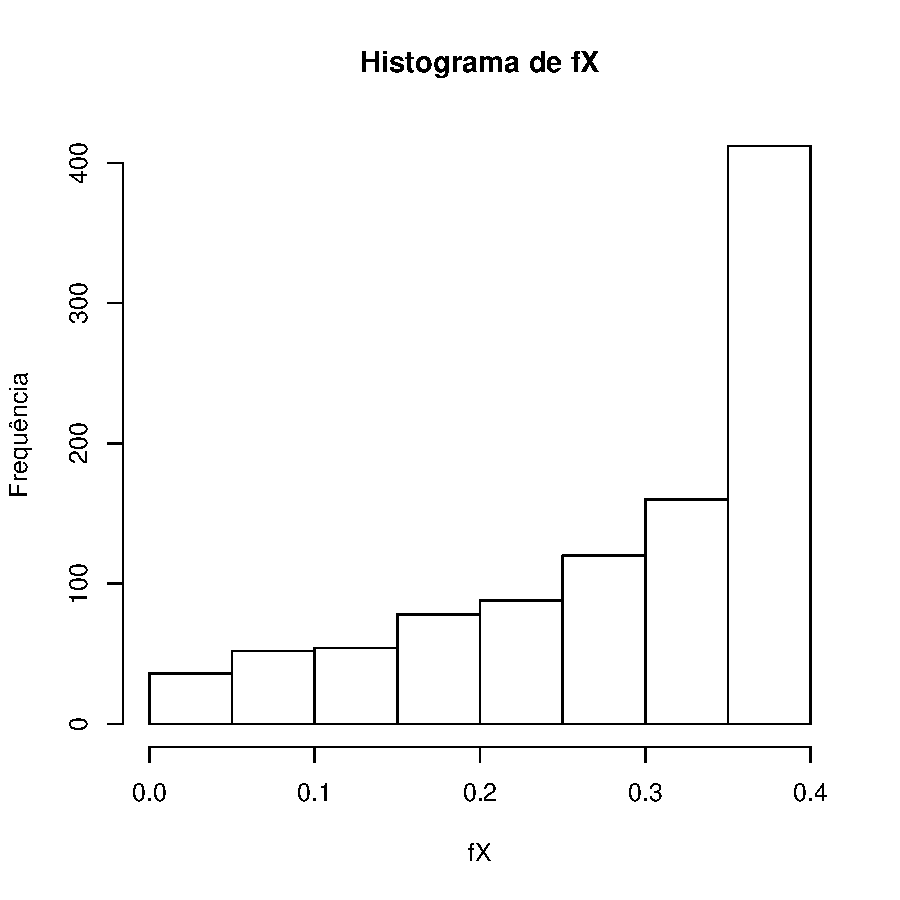
\includegraphics{transformacao-001}
\begin{Schunk}
\begin{Sinput}
> hist(fY,ylab="Frequência",main="Histograma de fY")
\end{Sinput}
\end{Schunk}
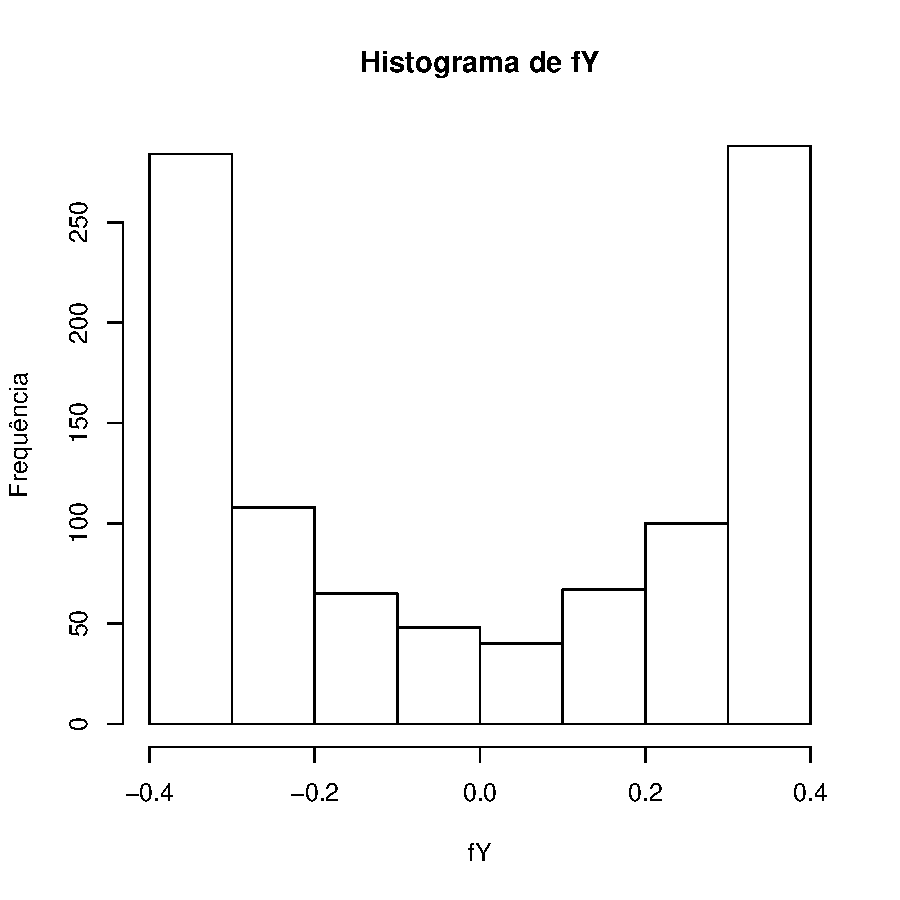
\includegraphics{transformacao-002}



      \item Para $Y = \frac{\sigma}{X-\mu}$\\

        $Y = g(X) = \frac{\sigma}{X-\mu}$, para $X \neq \mu$\\

        $g^{-1}(Y) = X = \frac{\sigma}{Y}+\mu$\\

        $\frac{d}{dy}g^{-1}(y) = \frac{d}{dy}(\frac{\sigma}{y}+\mu) = -\sigma y^{-2}$\\

        A função gaussiana é crescente para $X \leq \mu$ e decrescente para $X > \mu$.\\

        $f_Y(y) = f_X(g^{-1}(y))\frac{d}{dy}g^{-1}(y) = f_X(\frac{\sigma}{y}+\mu)(-\sigma y^{-2})$\\

        $f_Y(y) = \frac{1}{\sigma\sqrt{2\pi}}e^{-\frac{(\frac{\sigma}{y}+\mu-\mu)^2}{2\sigma^2}}(-\sigma y^{-2}) = \frac{1}{\sigma\sqrt{2\pi}}e^{-\frac{1}{2}(\frac{1}{y})^2}(-\sigma y^{-2})$\\

        $f_Y(y) = -\frac{1}{y^2\sqrt{2\pi}}e^{-\frac{1}{2y^2}}$\\      

        Esta é a expressão para $X \leq \mu$, isto é, crescente. Para $X > \mu$

        $f_Y(y) = \frac{1}{y^2\sqrt{2\pi}}e^{-\frac{1}{2y^2}}$\\
        
        Para demonstrar a transformação se usará $\sigma=1$ e $\mu=0$\\

\begin{Schunk}
\begin{Sinput}
> set.seed(236)
> sigma <- 1
> mu <- 0
> X <- rnorm(n=1000,mean=mu,sd=sigma)
> Ytrans <- function(y,mean=mu,sd=sigma){
+   ret <- NULL
+   yt <- (1/((y^2)*sqrt(2*pi)))*exp(-1/(2*y^2));
+   if(y<mean){
+     ret <- -yt
+   }else{
+     if(y>mean){
+       ret <- yt
+     }
+   }
+   return <- ret 
+ }
> fX <- dnorm(X,mean=mu,sd=sigma)
> fY <- sapply(X,Ytrans)
> fY<-subset(fY,fY!=0)
> hist(fX,ylab="Frequência",main="Histograma de fX")
\end{Sinput}
\end{Schunk}
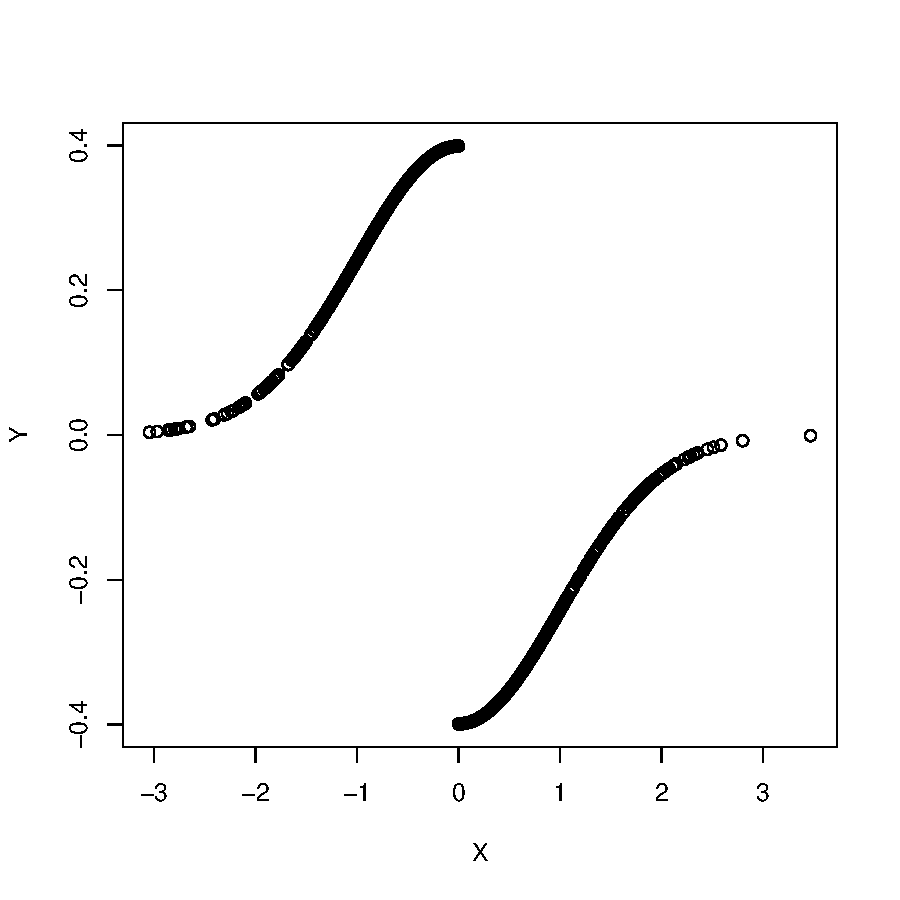
\includegraphics{transformacao-003}

\begin{Schunk}
\begin{Sinput}
> hist(x=fY,ylab="Frequência",main="Histograma de fY")
\end{Sinput}
\end{Schunk}
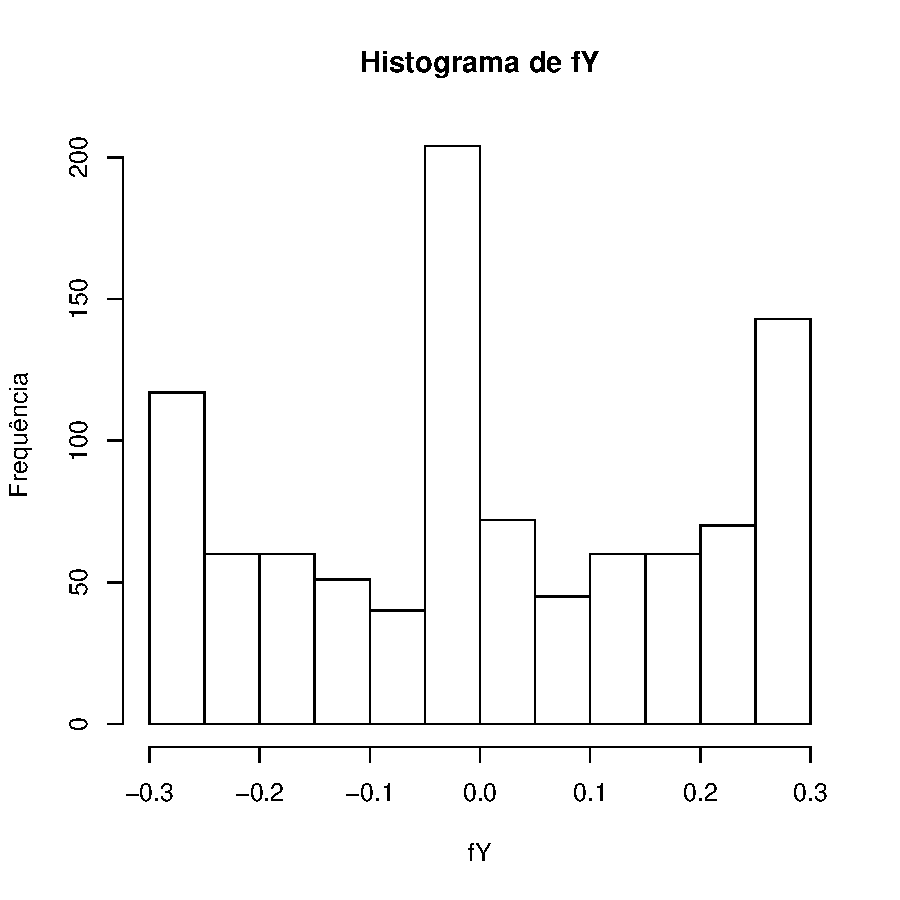
\includegraphics{transformacao-004}

      \item Para $Y = (\frac{X-\mu}{\sigma})^3$
      
        $Y = g(X) = (\frac{X-\mu}{\sigma})^3$ para $\sigma \neq 0$\\

        $g^{-1}(Y) = X = \sigma Y^{\frac{1}{3}}+\mu$\\

        $\frac{d}{dy}g^{-1}(y) = \frac{d}{dy}(\sigma y^{\frac{1}{3}}+\mu) = \frac{1}{3}\sigma y^{-\frac{2}{3}}$\\

        A função gaussiana é crescente para $X \leq \mu$ e decrescente para $X > \mu$.\\

        $f_Y(y) = f_X(g^{-1}(y))\frac{d}{dy}g^{-1}(y) = f_X(\sigma y^{\frac{1}{3}}+\mu)(\frac{1}{3}\sigma y^{-\frac{2}{3}})$\\

        $f_Y(y) = \frac{1}{\sigma\sqrt{2\pi}}e^{-\frac{(\sigma y^{\frac{1}{3}}+\mu-\mu)^2}{2\sigma^2}}(\frac{1}{3}\sigma y^{-\frac{2}{3}}) = y^{-\frac{2}{3}}\frac{1}{3\sqrt{2\pi}}e^{-\frac{1}{2}y^{\frac{2}{3}}}$\\ 

        A função gaussiana é crescente para $X \leq \mu$ e decrescente para $X > \mu$.\\

        $f_Y(y) = -y^{-\frac{2}{3}}\frac{1}{3\sqrt{2\pi}}e^{-\frac{1}{2}y^{\frac{2}{3}}}$\\ 
        
        Para demonstrar a transformação se usará $\sigma=1$ e $\mu=0$\\

\begin{Schunk}
\begin{Sinput}
> set.seed(236)
> sigma <- 1
> mu <- 0
> X <- rnorm(n=1000,mean=mu,sd=sigma)
> Ytrans <- function(y,mean=mu,sd=sigma){
+   yt <- -(y^(-2/3))*(1/(3*sqrt(2*pi)))*exp(-(1/2)*y^(2/3))
+   return <- ifelse(y>mean,yt,-yt)
+ }
> fX <- dnorm(X,mean=mu,sd=sigma)
> fY <- Ytrans(X)
> hist(fX,ylab="Frequência",main="Histograma de fX")
\end{Sinput}
\end{Schunk}
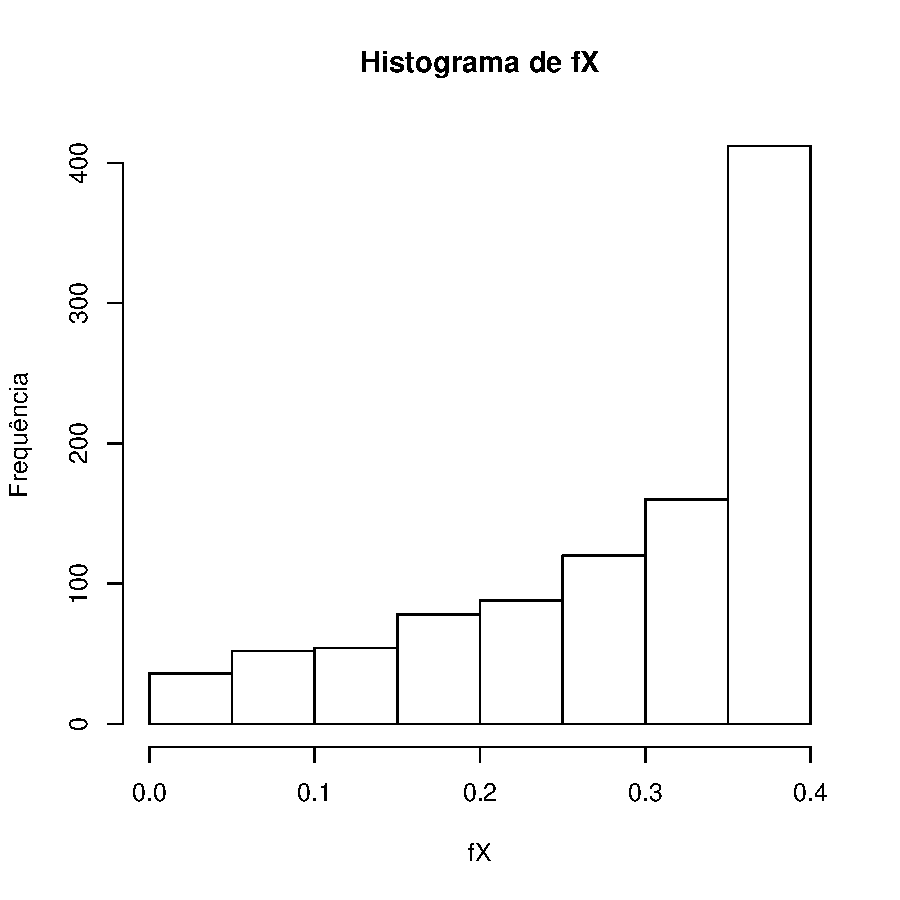
\includegraphics{transformacao-005}

\begin{Schunk}
\begin{Sinput}
> hist(x=fY,ylab="Frequência",main="Histograma de fY")
> 
\end{Sinput}
\end{Schunk}
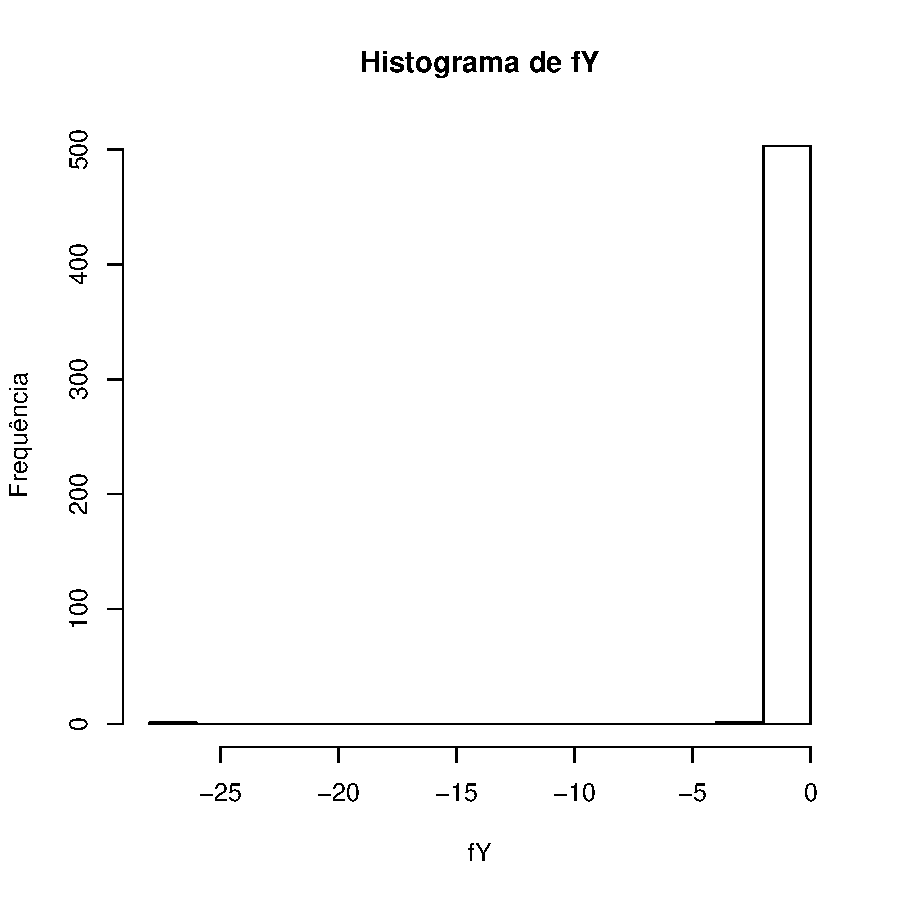
\includegraphics{transformacao-006}


    \end{enumerate}
  \item $X \sim \varepsilon(1)$, transformar em $Y = X^p$, para $p \neq 0$ 
  
  A função exponencial tem por função de distribuição\\
  
  $f(x) = \lambda e^{-\lambda x}$\\
  
  Como solicitado
  
  $Y = g(X) = X^p$\\
  
  $g^{-1}(Y) = X = Y^\frac{1}{p}$\\
  
  $\frac{d}{dy}g^{-1}(y) = \frac{d}{dy}y^\frac{1}{p} = \frac{1}{p}y^\frac{1-p}{p}$\\
  
  Como a função de distribuição exponencial é definida para $X \geq 0$ e é unicamente decrescente, pode-se indicar\\
  
  $f_Y(y) = -f_X(g^{-1}(y))\frac{d}{dy}g^{-1}(y) = -f_X(y^\frac{1}{p})\frac{1}{p}y^\frac{1-p}{p}$\\
  
  $f_Y(y) = -(\lambda e^{-\lambda y^\frac{1}{p}})\frac{1}{p}y^\frac{1-p}{p}$\\
  
  Para demonstrar a transformação se usará $\lambda=1$ e $p=3$\\

\begin{Schunk}
\begin{Sinput}
> set.seed(236)
> lambda <- 1
> p <- -3
> X <- rexp(n=1000,rate=lambda)
> Ytrans <- function(y,rate=lambda,ep=p){
+   return <- -rate*exp(-rate*y^(1/ep))*(1/ep)*y^((1-p)/p)
+ }
> fX <- dexp(X,rate=lambda)
> fY <- Ytrans(X)
> hist(fX,ylab="Frequência",main="Histograma de fX")
\end{Sinput}
\end{Schunk}
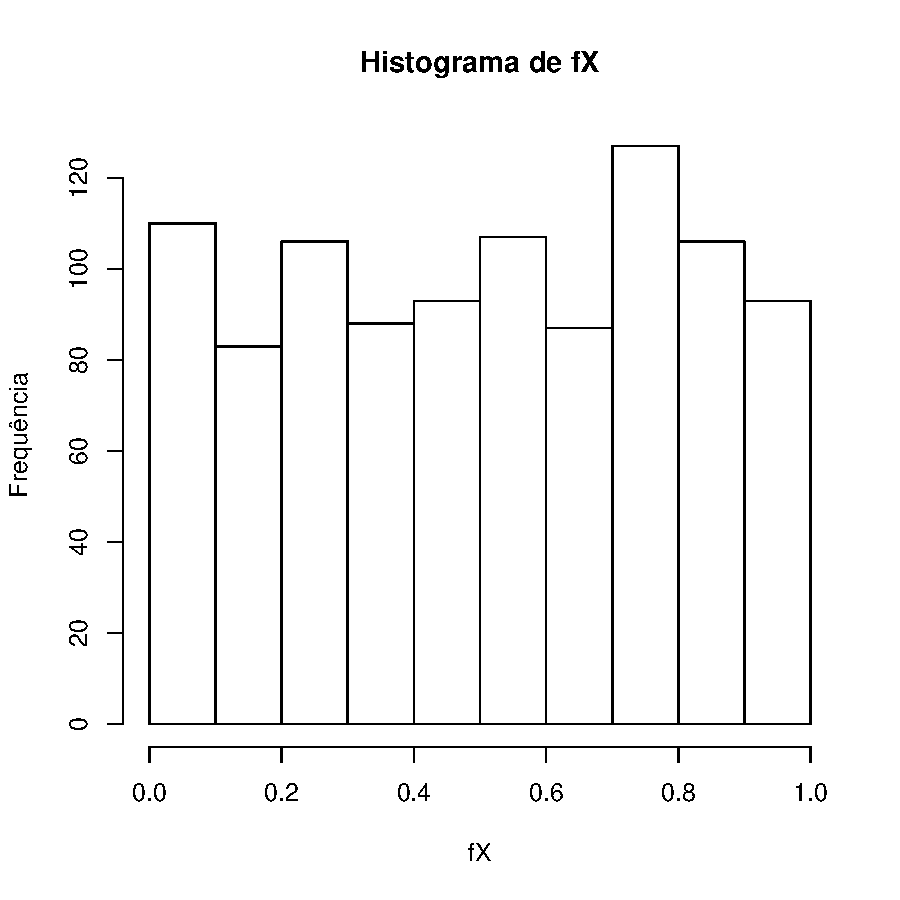
\includegraphics{transformacao-007}

\begin{Schunk}
\begin{Sinput}
> hist(x=fY,ylab="Frequência",main="Histograma de fY")
> 
\end{Sinput}
\end{Schunk}
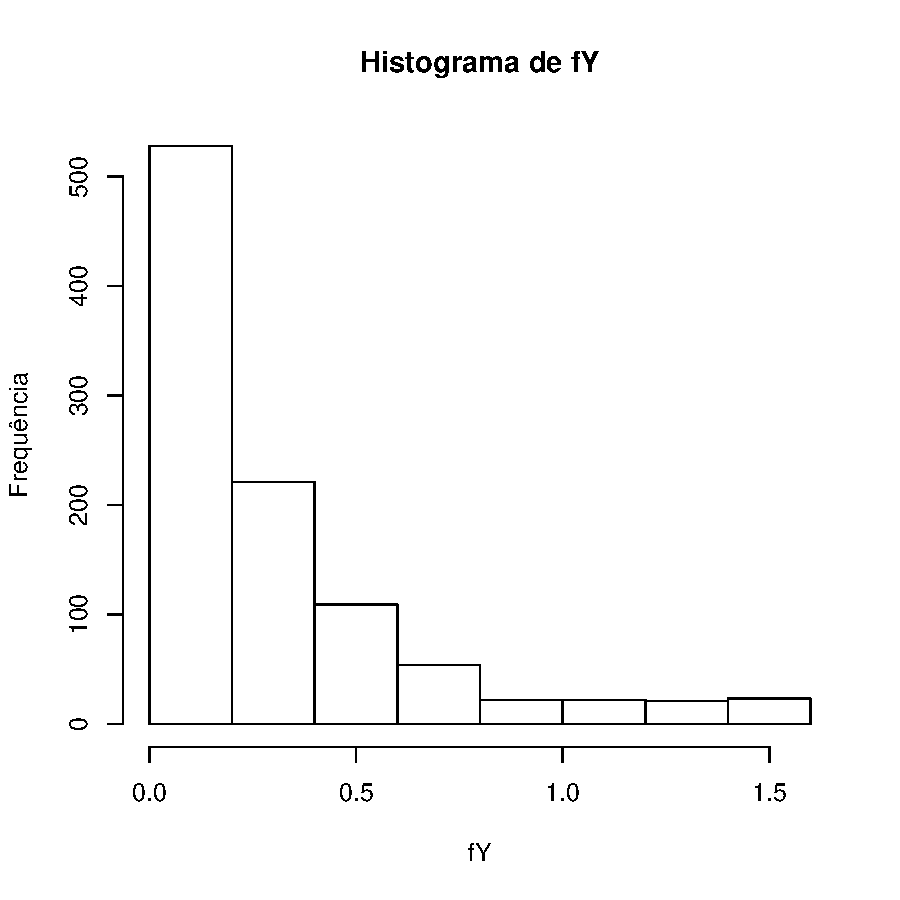
\includegraphics{transformacao-008}


  
  \item $X \sim U(0,1)$, transformar em $Y = aX+b$ 
\end{enumerate}

  A função de distribuição uniforme tem por expressão\\
  
  $f(x) = \frac{1}{b-a}I_{[a,b]}(x)$\\
  
  Isto a limita ao intervalo $[a,b]$ para indicada transformação\\
  
  $Y = g(X) = aX+b$\\
  
  $g^{-1}(Y) = X = \frac{a}{Y}-b$\\
  
  $\frac{d}{dy}g^{-1}(y) = \frac{d}{dy}(\frac{a}{y}-b) = -ay^{-2}$\\
  
  Usando o resultado final da equação \ref{fYFYXP}\\
  
  $f_Y(y) = f_X(g^{-1}(y))\frac{d}{dy}g^{-1}(y) = f_X(\frac{a}{y}-b)(-ay^{-2})$\\
  
  $f_Y(y) = \frac{1}{b-a}(-ay^{-2}) = -\frac{a}{y^2(b-a)}$
  
\begin{Schunk}
\begin{Sinput}
> set.seed(236)
> a <- 1
> b <- 3
> X <- runif(n=1000,min=a,max=b)
> Ytrans <- function(y,min=a,max=b){
+   return <- -min/((y^2)*(max-min))
+ }
> fX <- dunif(X,min=a,max=b)
> fY <- Ytrans(X)
> hist(fX,ylab="Frequência",main="Histograma de fX")
\end{Sinput}
\end{Schunk}
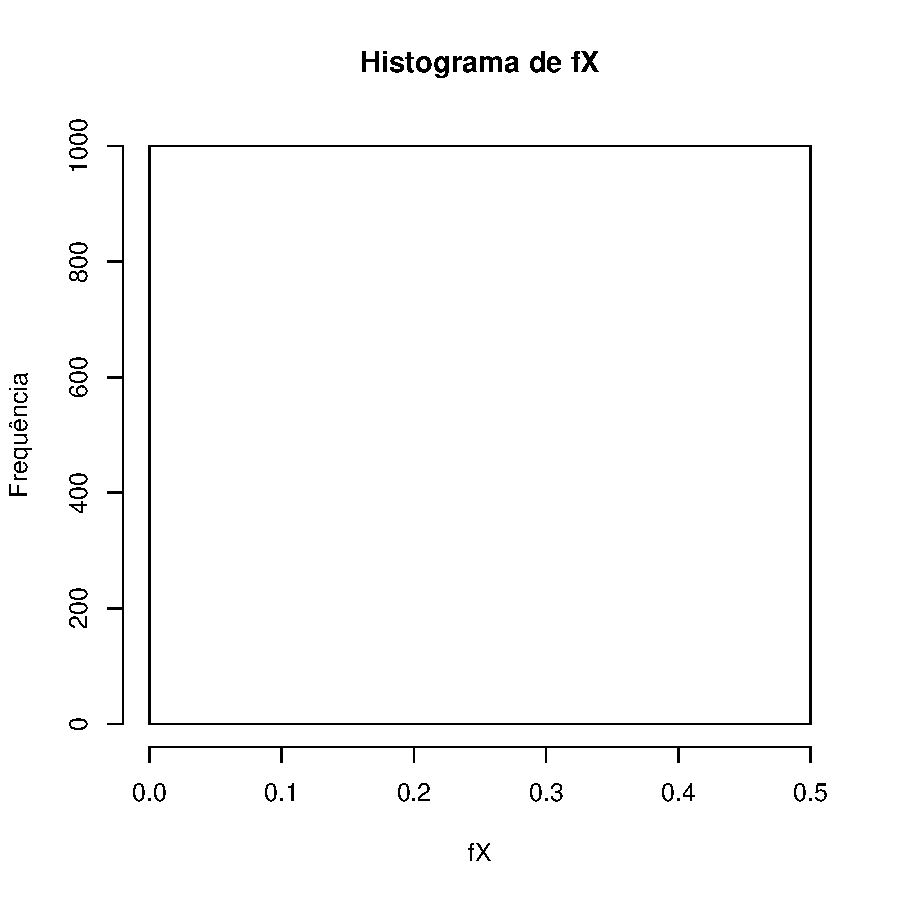
\includegraphics{transformacao-009}

\begin{Schunk}
\begin{Sinput}
> hist(x=fY,ylab="Frequência",main="Histograma de fY")
> 
\end{Sinput}
\end{Schunk}
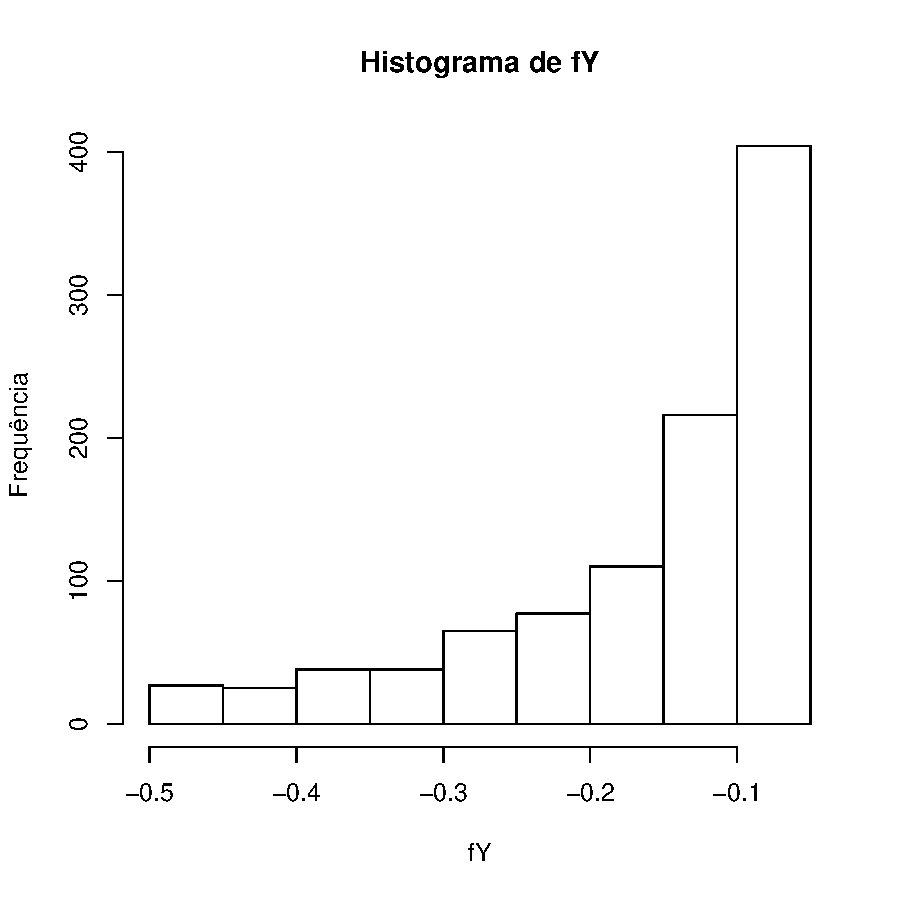
\includegraphics{transformacao-010}





\end{document}
